\subsection{Powering the Display}
The breadboard can be divided into 5 segments.  In each of the green segements, the pins are internally connected so as to have the same voltage.  Similarly, in the central segments, the pins in each column  are internally connected in the same fashion as the blue columns. 

\begin{problem}
	Plug the display to the breadboard in Fig. \ref{fig:breadboard}
\end{problem}
\begin{figure}[!h]
\begin{center}
\includegraphics[width=\columnwidth]{./figs/breadboard}
\end{center}
\caption{}
\label{fig:breadboard}
\end{figure}

The seven segment display in Fig. \ref{fig:sevenseg} has eight pins, $a, b, c, d, e, f, g$ and $dot$ that take an active LOW input, i.e.  the LED will glow only if the input is connected to ground.  Each of these pins is connected to an LED segment.  The $dot$ pin is  reserved for the $\cdot$ LED.  

%
%\begin{center}
	%\includegraphics[scale=1]{sevenseg}
%\end{center}

\begin{problem}
	Connect one end of the resistor to the COM pin of the display and the other end to an extreme pin of the breadboard.	
\end{problem}
%
%
%
\begin{figure}[!h]
\begin{center}
\resizebox {0.5\columnwidth} {!} {
\input{./figs/sevenseg.tex}
}
\end{center}
\caption{}
\label{fig:sevenseg}
\end{figure}

The Arduino Uno has some ground pins, analog input pins A0-A3 and digital pins D1-D13 that can be used for both input as well as output. It also has two power pins that can generate 3.3$V$ and 5$V$.  In the following exercises, only the GND, 5$V$ and digital pins will be used.
%
%\begin{center}
	%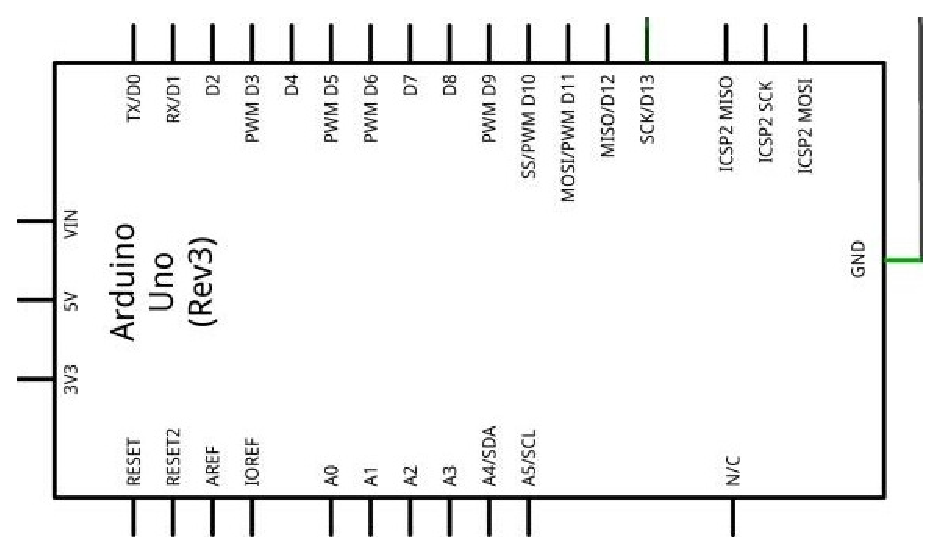
\includegraphics[scale=1]{arduino}
%\end{center}
%
\begin{problem}
	Connect the 5V pin of the arduino to an  extreme pin that is in the same segment as the 1K resistor pin. 
	\end{problem}	
\begin{problem}
	Connect the GND pin of the arduino to the opposite extreme pin of the breadboard
\end{problem}
\begin{problem}
	Connect the Arduino to the computer.
\end{problem}
\begin{problem}
	Connect the {\em dot} pin of the display to a pin in the same segment as the GND pin.  What do you observe?
\end{problem}
\subsection{Controlling the Display}
Fig. \ref{fig:sevenseg12} explains how to get decimal digits using the seven segment display. 
\begin{problem}
	Generate the number 1 on the display by connecting only the pins $b$ and $c$ to GND. 
\end{problem}	
\begin{problem}
	Repeat the above exercise to generate the number 2 on the display.
\end{problem}	
%
\begin{problem}
Table \ref{table:arduioport} summarizes the process of generating the decimal digits.  0 means connecting to ground and 1 means not connecting.  	Complete Table \ref{table:arduioport} for all numbers between 0-9.
\end{problem}	
\input{./figs/arduinoport}
%
%
\begin{figure}[!h]
\begin{center}
\resizebox {0.8\columnwidth} {!} {
\input{./figs/sevenseg12.tex}
}
\end{center}
\caption{}
\label{fig:sevenseg12}
\end{figure}
%
\begin{problem}
	Now generate all numbers between  0-9 on the display using the above table.
\end{problem}
%
%The 7447 IC helps in displaying decimal numbers on the seven segment display.  The $\bar{a}-\bar{g}$, pins of the 7447 IC are connected to the $a-g$ pins of the display. $V_{cc}$ should be connected to a 5V power source. The input pins of the decoder are A,B,C and D, with A being the lowest significant bit (LSB) and D being the most significant bit (MSB).  For example, the number 5 is visible on the display when the A,B,C and D inputs are the following.
%\begin{center}
%	\begin{tabular}{|c|c|c|c|c|}
%\hline
%D & C & B & A & Decimal
%\\ \hline
%0 & 1 & 0 & 1 & 5
%\\
%\hline
%\end{tabular}
%\end{center}
%
%%
%\begin{figure}
%\begin{center}
%\includegraphics[width=\columnwidth]{./figs/7447IC}
%\end{center}
%\caption{}
%\label{}
%\end{figure}
%
%%\begin{center}
%	%\includegraphics[scale=1.5]{7447IC}
%%\end{center}
%
%%
%\begin{problem}
%	Connect the 7447 IC decoder $\bar{a}-\bar{g}$ pins to the $a-g$ pins of the display respectively.
%\end{problem}
%\begin{problem}
%	Connect the $V_{cc}$ and GND pins of the decoder to the 5V supply and GND pins of the breadboard.
%\end{problem}
%\begin{problem}
%	Connect the A,B,C,D pins to pins in the GND extreme segment of the breadboard.  What do you observe.
%\end{problem}
%\begin{problem}
%	Now remove the D pin from the breadboard and observe the display output.
%\end{problem}
%\begin{problem}
%	Generate a table with A,B,C,D inputs and the equivalent decimal number output.
%\end{problem}
